% \documentclass[xetex, aspectratio=169, russian]{beamer}
\beamertemplatenavigationsymbolsempty
\setbeamertemplate{footline}[frame number]

\usepackage{fontspec}
\usepackage{polyglossia}
\usepackage[autostyle]{csquotes}
\setmainlanguage[babelshorthands]{russian}
\setotherlanguage{english}

\setmainfont{CMU Serif}
\setsansfont{CMU Sans Serif}
\setmonofont{CMU Typewriter Text}

\usepackage{booktabs}
\usepackage{multirow}
\usepackage{makecell}
\usepackage{ltablex}
\usepackage{paralist}
\keepXColumns
\renewcommand\theadfont{\normalsize}

\usepackage{fvextra}
\usepackage{xcolor}
\usepackage{textcomp}
\usepackage{graphicx}
\usepackage[edges]{forest}
\graphicspath{{../img/}}

\usepackage{mathtools}
\usepackage{amssymb}

\usepackage{covington}
\renewcommand*\glosslinetrans[1]{`#1'}

% Библиография
\usepackage[
    backend=biber,
    bibencoding=utf8,
    style=gost-authoryear,
    language=auto,
    autolang=other,
    clearlang=true,
    sortcites=true,
    movenames=false,
    minbibnames=3,
    maxbibnames=5
]{biblatex}

% Сортировка библиографии
\DeclareSourcemap{
    \maps[datatype=bibtex]{
        \map{
            \step[fieldsource=langid, match=russian, final]
            \step[fieldset=presort, fieldvalue={a}]
        }
        \map{
            \step[fieldsource=langid, notmatch=russian, final]
            \step[fieldset=presort, fieldvalue={z}]
        }
    }
}

% Убираем неразрывные пробелы перед двоеточием и точкой с запятой
\makeatletter

\renewcommand*{\addcolondelim}{%
    \begingroup%
    \def\abx@colon{%
        \ifdim\lastkern>\z@\unkern\fi%
        \abx@puncthook{:}\space}%
    \addcolon%
    \endgroup%
}

\renewcommand*{\addsemicolondelim}{%
    \begingroup%
    \def\abx@semicolon{%
        \ifdim\lastkern>\z@\unkern\fi%
        \abx@puncthook{;}\space}%
    \addsemicolon%
    \endgroup%
}

\makeatother

% Правка записей типа thesis, чтобы дважды не писался автор
\DeclareBibliographyDriver{thesis}{%
    \usebibmacro{bibindex}%
    \usebibmacro{begentry}%
    \usebibmacro{heading}%
    \newunit
    \usebibmacro{author}%
    \setunit*{\labelnamepunct}%
    \usebibmacro{thesistitle}%
    \setunit{\respdelim}%
    \newunit\newblock
    \printlist[semicolondelim]{specdata}%
    \newunit
    \usebibmacro{institution+location+date}%
    \newunit\newblock
    \usebibmacro{chapter+pages}%
    \newunit
    \printfield{pagetotal}%
    \newunit\newblock
    \usebibmacro{doi+eprint+url+note}%
    \newunit\newblock
    \usebibmacro{addendum+pubstate}%
    \setunit{\bibpagerefpunct}\newblock
    \usebibmacro{pageref}%
    \newunit\newblock
    \usebibmacro{related:init}%
    \usebibmacro{related}%
    \usebibmacro{finentry}%
}

% Короткое тире в интервалах страниц
\DefineBibliographyExtras{russian}{\protected\def\bibrangedash{\textendash}}

% Счётчик цитируемых источников
\usepackage{totcount}
\newtotcounter{citnum}
\AtEveryBibitem{\stepcounter{citnum}}

% Источники
\addbibresource{refs.bib}


% https://tex.stackexchange.com/a/30726
\newcommand\blfootnote[1]{%
  \begingroup
  \renewcommand\thefootnote{}\footnote{#1}%
  \addtocounter{footnote}{-1}%
  \endgroup
}

\title[]{Синтаксис}

\begin{document}


\frame{\titlepage}

\section{Вопросы терминологии}
\frame{\tableofcontents[currentsection]}

\begin{frame}
  \frametitle{Славянская ветвь}

  \begin{itemize}
    \item Южнославянская ветвь \begin{itemize}
      \item \ldots
      \item \alert<2->{Старославянский} $\rightarrow$ \alert<2->{Церковнославянский}
    \end{itemize}
    \item Восточнославянская ветвь \begin{itemize}
      \item \alert<2->{Древнерусский} \begin{itemize}
        \item \alert<2->{Старорусский} $\rightarrow$ Современный русский
        \item Украинский
        \item Белорусский
      \end{itemize}
      \item \alert<2->{Древненовгородский диалект}
      \item \ldots
    \end{itemize}
  \end{itemize}
\end{frame}

\begin{frame}
  \frametitle{Южнославянские языки}

  \begin{block}{Старославянский (Old Church Slavonic)}
    Первый литературный язык памятников славянской письменности 9--11~вв.
    Он же древнецерковнославянский, он же староболгарский, он же Жора\ldots
  \end{block}

  \begin{block}<2->{Церковнославянский (Church Slavonic)}
    Кодифицированный вариант старославянского языка, используемый для богослужения.
    Дожил до наших дней, преподается в духовных семинариях.
  \end{block}

  \vfill

  \begin{itemize}
    \item<3-> У обоих языков одинаковые ISO-коды
    \item<3-> Еще больше терминологическую ситуацию запутывают \textit{изводы}
  \end{itemize}
\end{frame}

\begin{frame}
  \frametitle{Восточнославянские языки}

  \begin{block}{Древнерусский (Old East Slavic)}
    Язык восточнославянской этнической общности. Материал~--- устная речь и~светская литература.
    В 14--15~вв.\ выделились украинский и белорусский.
  \end{block}

  \begin{block}<2->{Старорусский (Middle Russian)}
    Древнерусский язык в период 14--17~вв.\
    Соответствует этапу от распада общеславянского единства до формирования русского литературного языка.
  \end{block}
\end{frame}

\begin{frame}
  \frametitle{Корпуса исторические vs диахронические}

  \begin{block}{Исторический корпус}
    Корпус текстов на исторической разновидности современного языка или на древнем языке.
    $\sim$~Общеязыковой корпус
  \end{block}

  \begin{block}{Диахронический корпус}
    Корпус текстов на нескольких исторических разновидностях одного языка.
    $\sim$~Специальный корпус
  \end{block}

  \blfootnote{\autocite[242]{meyer:2006}}
\end{frame}

\section{Морфологически размеченные корпуса}

\subsection{Исторические подкорпуса НКРЯ}
\frame{\tableofcontents[currentsection,currentsubsection]}

\begin{frame}
  \frametitle{Древнерусский корпус}
  \framesubtitle{Наполнение}

  Тексты XI--XIV~вв., 500~тыс. с/у

  \begin{itemize}
    \item повести, летописи
    \item «публицистическая» литература
    \item небольшой массив церковнославянских памятников
  \end{itemize}

  \blfootnote{\autocite{sichinava:2014}}
  \blfootnote{\autocite{mishina_pichkhadze:2015}}
\end{frame}

\begin{frame}
  \frametitle{Древнерусский корпус}
  \framesubtitle{Разметка}

  \begin{block}{Морфология}
    Ручная разметка с обращением к базе прецедентов
  \end{block}

  \begin{block}{Дополнительная разметка}
    \begin{itemize}
      \item ударные и клитические формы
      \item филологическая адресация по номеру листа и строки
      \item ономастические, текстологические пометы
      \item для переводных памятников~--- перевод на греческий
    \end{itemize}
  \end{block}
\end{frame}

\begin{frame}
  \frametitle{Корпус берестяных грамот}
  \framesubtitle{\url{http://gramoty.ru/birchbark/}}

  \centering
  \begin{figure}[b]
    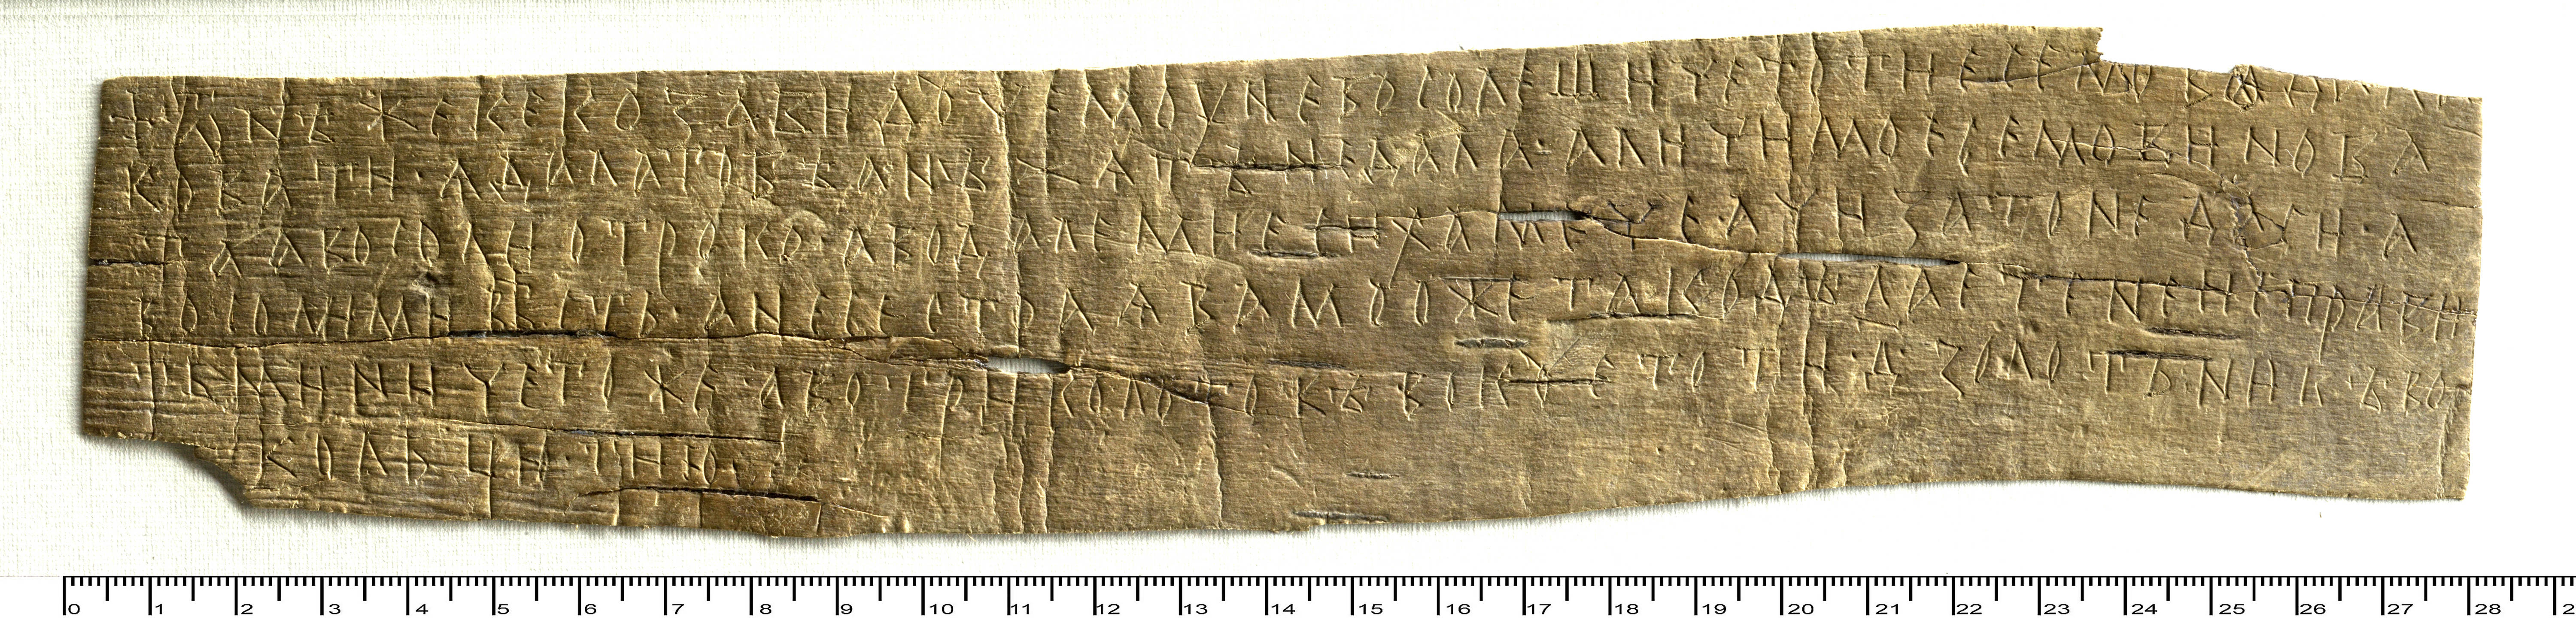
\includegraphics[width=.9\textwidth]{photo_novgorod_0644_1.jpg_thumb-large}
  \end{figure}

  \begin{figure}[t]
    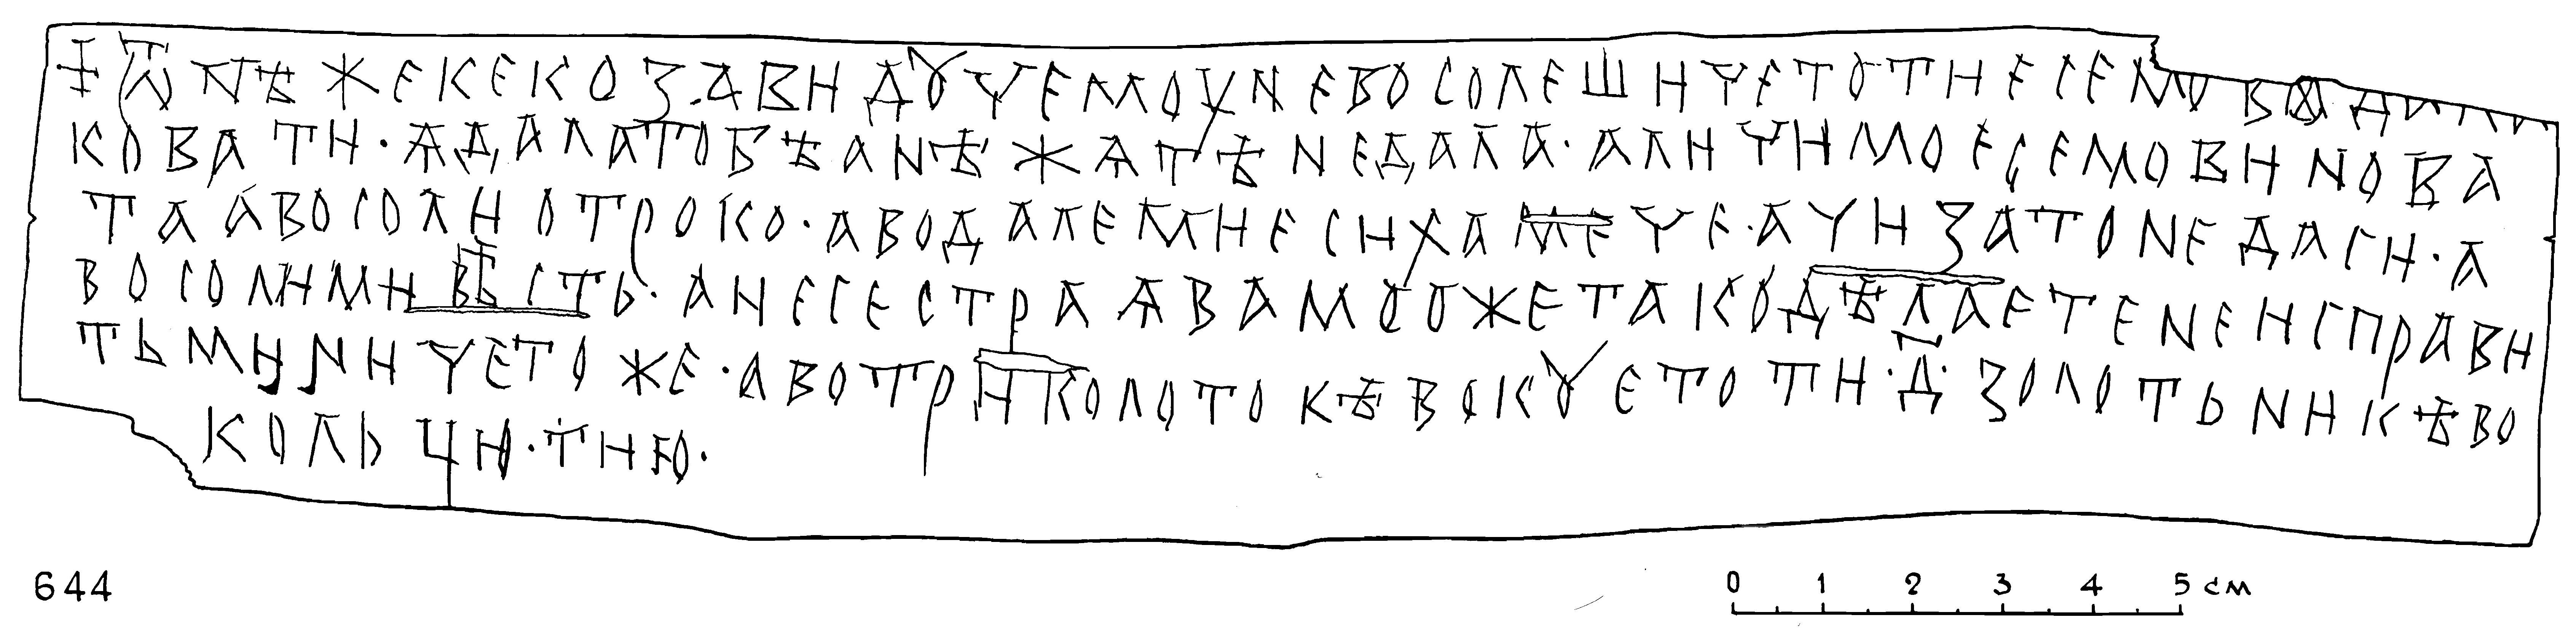
\includegraphics[width=.9\textwidth]{drawing_novgorod_0644_1}
  \end{figure}
\end{frame}

\begin{frame}
  \frametitle{Корпус берестяных грамот}

  \begin{itemize}
    \item $\sim$600 берестяных грамот, 20~тыс.\ с/у
    \item корпус не пополнялся с 2012~г.
    \item планируется обновление + интеграция с базой данных по эпиграфике
  \end{itemize}

  \blfootnote{\autocite{sichinava_dyshkant:2020}}
\end{frame}

\begin{frame}
  \frametitle{Церковнославянский подкорпус}
  \framesubtitle{Наполнение}

  \begin{itemize}
    \item XVII--XX~вв., 4,7~млн с/у
    \item Тексты, созданные уже в период книгопечатания
    \item 60\,\%~--- используемые в современной богослужебной практике
  \end{itemize}

  \blfootnote{\autocite{polyakov:2015}}
\end{frame}

\begin{frame}
  \frametitle{Церковнославянский подкорпус}
  \framesubtitle{Пример грамматической модели}

  \begin{table}
    \small
    \begin{tabularx}{\textwidth}{XXXXX}
      \toprule
      \thead{Парадигма} & \thead{N1t} & \thead{N1t*} & \thead{N1j} & \thead{N1k}   \\ \midrule\midrule
      \textit{Пример}   & рабъ        & сонъ         & конь        & отрокъ        \\ \midrule
      \textit{Основа}   & раб+ъ       & со*н+ъ       & кон+ь       & отро(к|ц|ч)+ъ \\ \midrule
      sg,nom            & ъ           & 2ъ           & ь           & ъ             \\ \midrule
      sg,gen            & а           & а            & я           & а             \\ \midrule
      sg,voc            & е           & е            & ю           & 3е            \\ \midrule
      pl,acc            & ы/=gen      & ы/=gen       & и/=gen      & ы/=gen        \\ \midrule
      pl,loc            & ѣхъ         & ѣхъ          & ехъ         & 2ѣхъ          \\ \midrule
      du,dat/ins        & ома         & ома          & ема         & ома           \\ \bottomrule
    \end{tabularx}
  \end{table}
\end{frame}

\begin{frame}
  \frametitle{Старорусский корпус}
  \framesubtitle{Наполнение}

  \begin{itemize}
    \item XV--XVII~вв., 7~млн с/у
    \item Летописи, повести, деловые документы\ldots
    \item «Огромный объем текстов и их орфографическая и языковая пестрота»
  \end{itemize}

  \blfootnote{\autocite{lyashevskaya:2016}}
\end{frame}

\begin{frame}
  \frametitle{Старорусский корпус}
  \framesubtitle{Гибридный морфологический анализ}

  \begin{block}{Первый подход}
    Адаптируем грамматический словарь для церковнославянского
  \end{block}

  \begin{block}<2->{Второй подход}
    \begin{enumerate}
      \item Размечаем как будто современный русский (MyStem и TreeTagger)
      \item Все, что не разметилось, смотрим в базе древнерусских прецедентов
    \end{enumerate}
  \end{block}
\end{frame}

\subsection{Манускрипт}
\frame{\tableofcontents[currentsection,currentsubsection]}

\begin{frame}
  \frametitle{Наполнение}

  \begin{itemize}
    \item 140 ц.-сл.\ (включая 5 на глаголице) и др.-р.\ текстов, 3,5~млн с/у
    \item активные количественные и статистические исследования
  \end{itemize}

  \blfootnote{\autocite{baranov:2010}}
\end{frame}

\begin{frame}
  \frametitle{Параметры морфологических единиц}

  \begin{table}
    \small
    \begin{tabularx}{\textwidth}{p{2.5cm}XX}
      \toprule
      \thead{Часть речи} & \thead{Параметры типов изменения} & \thead{Параметры окончаний} \\ \midrule\midrule
      \textit{сущ} & род & число, падеж \\ \midrule
      \textit{прил} & членность, разряд & род, число, падеж \\ \midrule
      \textit{гл} & наклонение & изменяемость, время, число, лицо \\ \midrule
      \textit{прич} & \textit{гл} $+$ время, залог, членность & \textit{гл} + род, падеж \\ \bottomrule
    \end{tabularx}
  \end{table}
\end{frame}

\subsection{СКАТ}
\frame{\tableofcontents[currentsection,currentsubsection]}

\begin{frame}
  \frametitle{}

  ...

  \blfootnote{\autocite{azarova_alexeeva:2013}}
  \blfootnote{\autocite{content_structuring:2021}}
\end{frame}

\section{Трибанки}

\subsection{Семейство проектов PROIEL}
\frame{\tableofcontents[currentsection,currentsubsection]}

\begin{frame}
  \frametitle{PROIEL}
  \framesubtitle{\url{http://dev.syntacticus.org/}}

  Корпус новозаветных текстов на различных древних языках: древнегреческом, латыни, готском, древнеармянском, старославянском. \linebreak

  По назначению специальный параллельный корпус для изучения прагматических феноменов: порядка слов, употребления артиклей и дискурсивных частиц и др. \linebreak

  На ст.-сл.~--- Мариинское Евангелие из Corpus Cyrillo-Methodianum Helsingiense, 57~тыс.\ с/у. Сконвертирован в UD (единственный текст из раздела Old Church Slavonic).

  \blfootnote{\autocite{haug_johndal:2008}}
\end{frame}

\begin{frame}
  \frametitle{TOROT}
  \framesubtitle{\url{https://nestor.uit.no/}}

  \begin{block}{Наполнение}
    \begin{itemize}
      \item ст.-сл.~--- 160~тыс.\ с/у
      \item др.-р.~--- 85~тыс.\ с/у
      \item ст.-р.~--- 60~тыс.\ с/у
    \end{itemize}
  \end{block}

  \vfill

  \begin{itemize}
    \item Тексты из разных источников
    \item Все переведено в Юникод, сконвертировано в PROIEL XML
    \item Др.-р.\ сегмент переведен в UD
  \end{itemize}

  \blfootnote{\autocite{eckhoff_berdicevskis:2015}}
\end{frame}

\subsection{НКРЯ}
\frame{\tableofcontents[currentsection,currentsubsection]}

\begin{frame}
  \frametitle{Старорусский корпус}

  \centering
  Небольшой кусочек (34~тыс.\ с/у)

  \blfootnote{\autocite{lyashevskaya:2019}}
\end{frame}

\section{Итоги}
\frame{\tableofcontents[currentsection]}

\begin{frame}
  \frametitle{Морфологически размеченные корпуса}

  \begin{table}[t]
    \small
    \begin{tabularx}{\linewidth}{XXXXXX}
      \toprule
      \thead{Корпус} & \thead{Охват, \\ вв.} & \thead{Объем, \\ с/у} & \thead{Разметка} & \thead{Дизамби"= \\ гуация} & \thead{Леммати"= \\ зация} \\ \midrule\midrule
      НКРЯ: \linebreak др.-р. & XI--XIV & 500~тыс. & Ручная & Есть & Есть \\ \midrule
      НКРЯ: \linebreak б.~гр. & XI--XV & 20~тыс. & Ручная & Есть & Есть \\ \midrule
      СКАТ & XV--XVII & 500~тыс. & Ручная & Есть & Есть \\ \midrule
      НКРЯ: \linebreak ц.-сл. & XVII--XX & 4,7~млн & Словарная & Нет & Есть \\ \midrule
      НКРЯ: \linebreak ст.-р. & XV--XVII & 7~млн & Словарная & Нет & Нет \\ \midrule
      Манускрипт & X--XIV & 3,5~млн & Словарная & Есть & Есть \\ \bottomrule
    \end{tabularx}
  \end{table}
\end{frame}

\begin{frame}
  \frametitle{Проблемы}

  \begin{itemize}
    \item Closed source. К корпусам, где больше всего данных (НКРЯ и Манускрипт), нет открытого полнотекстового доступа
    \item Цифровизация как неизбежность. Что (какие лингвистические единицы) и как (к вопросу о кодировке) представлять~--- все решают по-своему
  \end{itemize}
\end{frame}
